\scanpage{117}
\mspage{3}

Les notations introduites sont telles qu'elles gardent un sens pour toute carte triangulaire ``polarisée'' de type $\{0,1,\infty\}$, sans que celle\deleted{\unsure{qui est la}} \inserted{-ci soit} nécessairement : la subdivision barycentrique d'une carte $X$, condition qui s'exprime par la \deleted{\unsure{condition}} \inserted{dernière} relation
\[
\deleted{\unsure{\tau_0}}\qquad (\tau_0\tau_\infty)^2=1\qquad\text{i.e.}\quad\rho_1^2=1
\]
dans $(4)$ (qu'on abandonne donc par la suite) et qui signifie aussi que les \deleted{points} \inserted{sommets} de type $1$ sont d'ordre réduit $2$ (d'ordre ordinaire $4$), ou encore que $\tau_0\tau_\infty(r)=\tau_\infty\tau_0(r)$ pour tout $r$. Dans le cas général, $\rho_1$ est donc une op. qui ne joue plus un rôle particulier p.r. à $\rho_0,\rho_\infty$ : c'est la rotation ``d'un cran'' de $r$ autour du sommet de type $1$, dans le \deleted{\unsure{demi-tour défini}} \inserted{sens défini} par l'orientation de $r$.

On introduit
\[
(13)\qquad\left\{
\begin{aligned}
\Lambda_r^i&=(\lambda_{\unsure{\tau_{i+1}r|\tau_{i+1}}}^i)^{-1}\lambda_r^i:R_r^{i,i+1}\mathrel{\unsure{-|\longrightarrow}} R_{\tau_{i+1}(r)}^{i,i+1}\\
\Lambda_r^{\prime i}&=\lambda_{\unsure{\sigma_{i-1}(r)|\tau_{i-1}(r)}}^i(\lambda_r^i)^{-1}:R_r^{i,i-1}\mathrel{\unsure{-|\longrightarrow}} R_{\tau_{i-1}(r)}^{\unsure{i-1|i,i-1}}
\end{aligned}\right.
\]
rotation d'un double ``cran'' autour du sommet de type $i$ de $r$, à partir du sommet proche de type $(i,i+1)$, \inserted{resp. $(i,i-1)$}, dans le sens de rotation donné par l'orientation de $r$. \inserted{resp. en sens opposé} On a les relations

\figure{
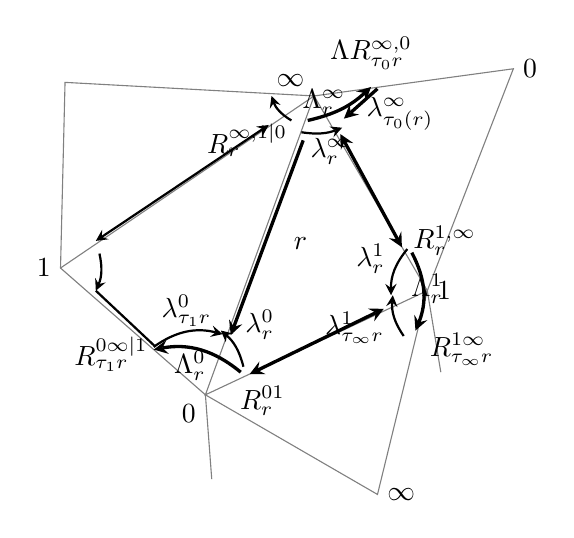
\begin{tikzpicture}[scale=1.15,>=stealth]
\coordinate (A) at (1.75,0.95);\coordinate (B) at (4.2,2.1);\coordinate (C) at (2.95,4.25);
\coordinate (D) at (0.15,2.35);\coordinate (E) at (5.15,4.55);\coordinate (F) at (3.65,-0.15);\coordinate (G) at (0.2,4.4);
\draw[gray] (G)--(C)--(E)--(B)--(F)--(A)--(D)--cycle;
\draw[gray] (A)--(B)--(C)--cycle (D)--(C) (A)--(1.82,0.02) (B)--(4.35,1.2);
\draw[very thick,->] (2.83,3.76)--(2.03,1.61);
\draw[very thick,<->] (2.24,1.18)--(3.72,1.9);
\draw[very thick,<->] (3.92,2.58)--(3.24,3.83);
\draw[thick,<->] (0.54,2.65)--(2.45,3.93);
\draw[thick,->] (0.58,2.51) to[bend left=18] (0.54,2.10);
\draw[thick] (0.54,2.10)--(1.20,1.48);
\draw[thick,->] (2.17,1.26) to[bend right=18] (1.92,1.66);
\draw[thick,->] (1.18,1.48) to[bend left=25] (1.94,1.62);
\draw[very thick,->] (2.14,1.20) to[bend right=25] (1.18,1.45);
\draw[thick,->] (3.98,2.56) to[bend right=20] (3.80,2.05);
\draw[thick,->] (3.94,1.60) to[bend left=20] (3.82,2.05);
\draw[very thick,->] (4.03,2.52) to[bend left=25] (4.07,1.66);
\draw[thick,->] (2.81,3.85) to[bend right=15] (3.26,3.90);
\draw[thick,->] (2.70,3.98) to[bend left=20] (2.48,4.25);
\draw[very thick,->] (2.88,3.98) to[bend right=15] (3.58,4.35);
\draw[very thick,->] (3.65,4.33)--(3.28,4.00);
\node[below left] at (A) {$0$};\node[right] at (B) {$1$};\node[above left] at (C) {$\infty$};
\node[left] at (D) {$1$};\node[right] at (E) {$0$};\node[right] at (F) {$\infty$};\node at (2.8,2.62) {$r$};
\node[below] at (2.38,1.15) {$R_r^{01}$};
\node[left] at (1.22,1.40) {$R_{\tau_1r}^{0\unsure{\infty|1}}$};
\node at (1.54,1.88) {$\lambda_{\tau_1r}^0$};\node at (1.58,1.27) {$\Lambda_r^0$};\node at (2.35,1.72) {$\lambda_r^0$};
\node[right] at (3.94,2.65) {$R_r^{1,\infty}$};\node[right] at (4.12,1.45) {$R_{\tau_\infty r}^{1\infty}$};
\node[left] at (3.84,2.45) {$\lambda_r^1$};\node[left] at (3.83,1.69) {$\lambda_{\tau_\infty r}^1$};\node at (4.20,2.12) {$\Lambda_r^1$};
\node[left] at (2.76,3.76) {$R_r^{\infty,\unsure{1|0}}$};\node[above] at (3.58,4.44) {$\deleted{\unsure{\Lambda}}R_{\tau_0r}^{\infty,0}$};
\node at (3.13,3.64) {$\lambda_r^\infty$};\node at (3.90,4.05) {$\lambda_{\tau_0(r)}^\infty$};\node at (3.06,4.18) {$\Lambda_r^\infty$};
\end{tikzpicture}
}
\[
(14)\qquad \boxed{\Lambda_r^i\Lambda_{\tau_{i+1}(r)}^i=1}\qquad
\boxed{\Lambda_r^{\prime i}\Lambda_{\tau_{i-1}(r)}^{\prime i}=1}.
\]

\mspage{116}
